\chapter{Work Done}

\section{Experimental Framework}

\begin{figure}[htb]
\centering
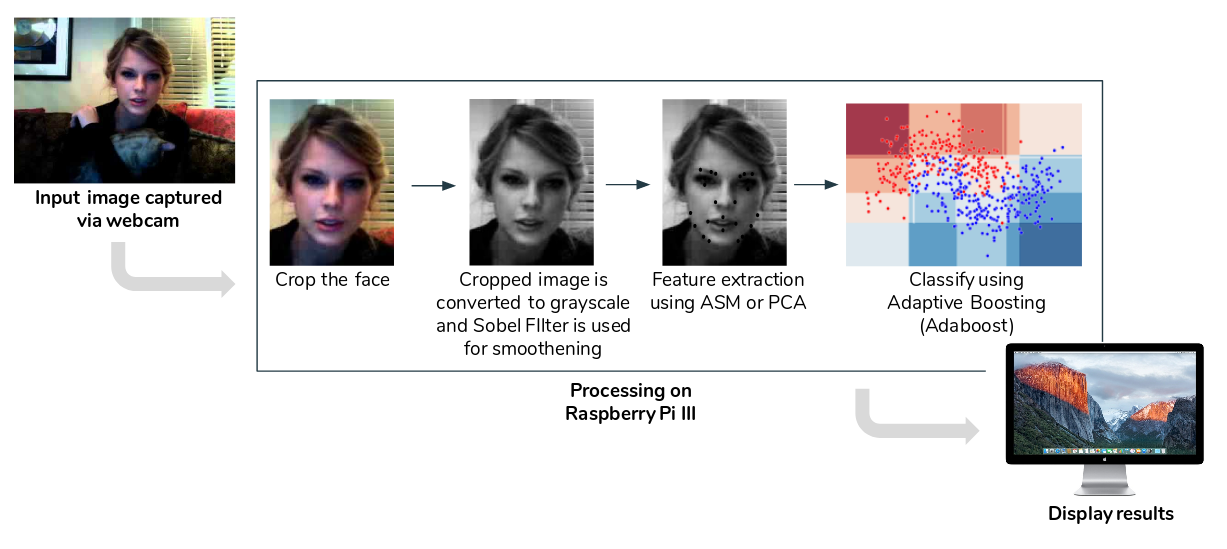
\includegraphics[scale=0.35]{images/model}
\caption{Flow of control from Input to Output to detect `Emotions' (real-time)}
\label{fig:model}
\end{figure}

\section{Work Done (Mid-March 2018)}

\subsection{Capturing Input via Webcam (Linux)}
\begin{lstlisting}[language=python]
pygame.camera.init()
cam = pygame.camera.Camera("/dev/video0", (640, 640))
cam.start()
image = cam.get_image()
pygame.image.save(image, localpath)

try:
    conn = sftp.Connection(host='10.42.0.178', username='pi', password='raspberry')
    conn.put(localpath, remotepath)
    conn.close()
except Exception, e:
    print str(e)
\end{lstlisting}

\subsection{Preprocessing the Image (RPi): Facial Region Extraction}
\begin{lstlisting}[language=python]
def convertToRGB(image):
    return cv2.cvtColor(image, cv2.COLOR_BGR2RGB)

image = cv2.imread(filename)
grayImage = cv2.cvtColor(image, cv2.COLOR_BGR2GRAY)
plt.imshow(grayImage, cmap = "gray")

haarFaceCascade = cv2.CascadeClassifier('training/haarcascade_frontalface_alt.xml')

faces = haarFaceCascade.detectMultiScale(grayImage, scaleFactor = 1.1, minNeighbors = 5)
print "Number of faces found: %s" %(len(faces))

for (x, y, w, h) in faces:
    cv2.rectangle(image, (x, y), (x + w, y + h), (0, 255, 0), 2)
plt.imshow(convertToRGB(image))

def violaJones(filename, trainingFile, scaleFactor = 1.2):
    image = cv2.imread(image_directory + filename)
    grayImage = cv2.cvtColor(image, cv2.COLOR_BGR2GRAY)
    
    haarFaceCascade = cv2.CascadeClassifier(training_directory + trainingFile)
    faces = haarFaceCascade.detectMultiScale(grayImage, scaleFactor = scaleFactor, minNeighbors = 5)
    print "Number of faces found: %s" %(len(faces))

    deleteAllFiles(faces_directory)
    for (x, y, w, h) in faces:
        cv2.rectangle(image,(x, y),(x+w, y+h),(0, 255, 0),2)
        sub_face = image[y : y + h, x : x + w]
        
        faceFile=faces_directory + "face_" + str(y) + ".jpg"
        cv2.imwrite(faceFile, sub_face)
    image = convertToRGB(image)
    return image
\end{lstlisting}


\subsection{Preprocessing the Image (RPi): Sobel Filter}
\begin{lstlisting}[language=python]
image = cv2.imread(filename, cv2.IMREAD_GRAYSCALE)
laplacian = cv2.Laplacian(image, cv2.CV_64F)
sobelX = cv2.Sobel(image, cv2.CV_64F, 1, 0, ksize=5)
sobelY = cv2.Sobel(image, cv2.CV_64F, 0, 1, ksize=5)

def sobelYFilter(directory):
    deleteAllFiles(sobel_directory)
    filelist = [f for f in os.listdir(directory)]
    for f in filelist:
        filename = faces_directory + f

        image = cv2.imread(filename, cv2.IMREAD_GRAYSCALE)
        sobelY = cv2.Sobel(image, cv2.CV_64F, 0, 1, ksize=5)
        
        sobelFile = sobel_directory + f
        cv2.imwrite(sobelFile, sobelY)
        plt.imshow(sobelY)
\end{lstlisting}

\section{Results and Discussion}

\subsection{Capturing on Linux}
\begin{figure}[htb]
\centering
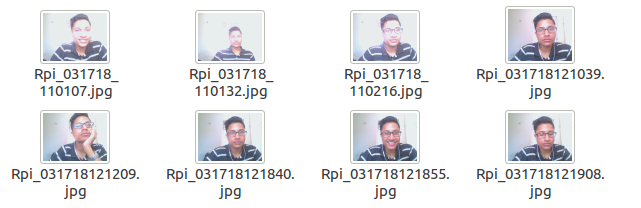
\includegraphics[scale=0.7]{images/capture}
\caption{Capturing through webcam in real-time (different illuminations and non-uniform conditions) with low resolution}
\label{fig:capture}
\end{figure}

\subsection{Viola-Jones on RPi3}
The facial image is detected by using Viola-Jones face detection technique. The integral image is developed by using Haar wavelet concept to detect the face. It consider the different intensity of values of adjacent rectangular regions. The different areas of face have different intensity. Face is detected and pointed by using rectangular box (then cropped). Refer figures \ref{fig:vj1}, \ref{fig:vj2}, \ref{fig:vj3} and \ref{fig:vj4}.

\begin{figure}[htb]
\centering
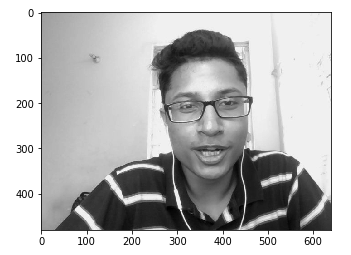
\includegraphics[scale=0.5]{images/vj_img1}
\caption{Converting the input image (from Linux) into grayscale}
\label{fig:vj1}
\end{figure}

\begin{figure}[htb]
\centering
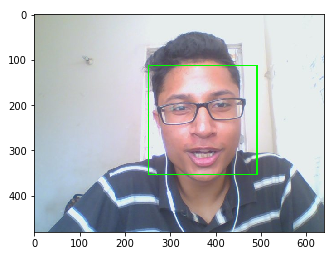
\includegraphics[scale=0.5]{images/vj_img2}
\caption{Face Detection using Haar-Cascade Classifier (of figure \ref{fig:vj1})}
\label{fig:vj2}
\end{figure}

\begin{figure}[htb]
\centering
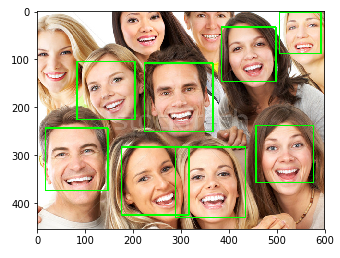
\includegraphics[scale=0.5]{images/vj_img3}
\caption{Capturing multiple faces using Viola-Jones Algorithm (Haar-Cascade)}
\label{fig:vj3}
\end{figure}

\begin{figure}[htb]
\centering
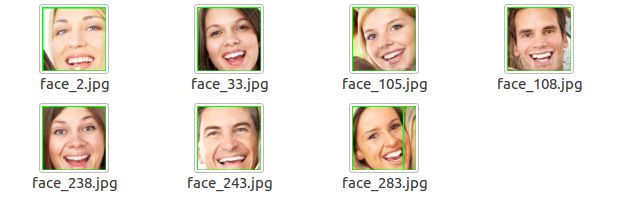
\includegraphics[scale=0.5]{images/vj_img4}
\caption{Crop the facial part and discard the rest of the image (of figure \ref{fig:vj3})}
\label{fig:vj4}
\end{figure}

\subsection{Image Processing on RPi3}
In image preprocessing, image is cropped according to required size and converted in gray image. This cropped image is used as input to Sobel filter for smoothing to remove the noise. Refer figures \ref{fig:ip1}, \ref{fig:ip2}.

\begin{figure}[htb]
\centering
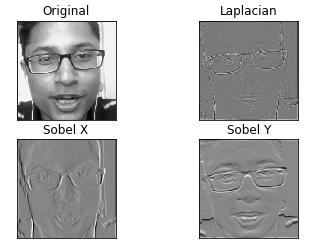
\includegraphics[scale=0.5]{images/ip_img1}
\caption{Crop the facial part and discard the rest of the image (of figure \ref{fig:vj2})}
\label{fig:ip1}
\end{figure}

\begin{figure}[htb]
\centering
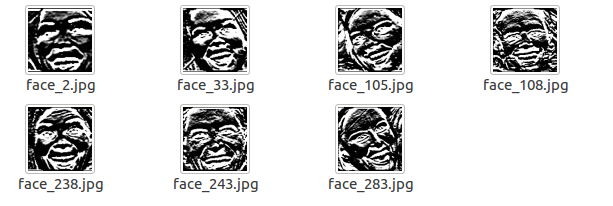
\includegraphics[scale=0.5]{images/ip_img2}
\caption{Crop the facial part and discard the rest of the image (of figure \ref{fig:vj4})}
\label{fig:ip2}
\end{figure}
\pagebreak

\section{Individual Contributions}

\begin{itemize}
\item Tushaar Gangarapu (15IT117) -- RPi3 Configuration, Capturing real-time input and directing it to RPi3 for pre-processing and emotion detection.
\item Bharath A. Kinnal (15IT114) -- Use the image obtained and run Haar-Cascade classifier to obtain `facial' region of the image.
\item Jyoti Prakash Sahoo (15IT213) -- Use the facial image and run `Sobel Filter' along \textit{Y-axis} and remove noise.
\end{itemize}